\documentclass[letterpaper, 10 pt, conference]{ieeeconf}

\IEEEoverridecommandlockouts                              % This command is only
% needed if you want to
% use the \thanks command
\overrideIEEEmargins

% The following packages can be found on http:\\www.ctan.org
\usepackage{graphics} % for pdf, bitmapped graphics files
\graphicspath{{images/}}
\usepackage{epsfig} % for postscript graphics files
\usepackage{mathptmx} % assumes new font selection scheme installed
\usepackage{times} % assumes new font selection scheme installed
\usepackage{amsmath} % assumes amsmath package installed
\usepackage{amssymb}  % assumes amsmath package installed
\usepackage{fixltx2e}
\usepackage{verbatim}
\usepackage{listings, lstautogobble}

\title{\LARGE \bf
	Concurrent Wait-Free Red Black Trees
}
\author{David Ferguson and Jacob Spigle% <-this % stops a space
	\thanks{$^{1}$D. Ferguson is a student at Department of Electrical Engineering and Computer Science, University of Central Florida, Orlando, Florida, 32816-2450 }%
	\thanks{$^{2}$J. Spigle is a student at Department of Electrical Engineering and Computer Science, University of Central Florida, Orlando, Florida, 32816-2450 %
}}

\begin{document}
	
	
	
	\maketitle
	\thispagestyle{empty}
	\pagestyle{empty}
	\lstset{language=C++, frame=single, basicstyle=\footnotesize\ttfamily, breaklines=true, stringstyle=\ttfamily, showstringspaces=false, frameround=ffff, autogobble=true, numbers=left,numberstyle=\tiny,numbersep=4pt}
	
	
	%%%%%%%%%%%%%%%%%%%%%%%%%%%%%%%%%%%%%%%%%%%%%%%%%%%%%%%%%%%%%%%%%%%%%%%%%%%%%%%%
	\begin{abstract}
		
		Our re-implementation of Natarajan, Savoie, and Mittal's wait-free algorithm \cite{c1} seeks to not only imitate the concurrent data structure presented, but also transform it into a transactional data structure using the RSTM library. We are implementing a concurrently managed red-black tree using wait-free algorithms designed and presented in \cite{c1}. We will be writing these algorithms using C++ as our programming language.  Concurrency during manipulation of a tree data structure is not plausible without additional (and creative) data structures because of the multiple instructions that rotations perform during the re-balancing of the tree. Using the techniques outlined in \cite{c1}, we will have a concurrent algorithm that makes progress, is linearizable, and correct. Experiments run by the authors of this implementation prove that their solution provides ``significantly better performance''\cite{c1} than other attempts that preceded it, including both attempts at concurrency and lock-based implementations.
		
	\end{abstract}
	
	
	\section{Introduction}
	This wait-free implementation of the Red Black tree data structure boasts search(), insert(), update(), and delete() functions, all executed utilizing single-word compare-and-swap instructions. The data structure's concurrent implementation employs the use of ``windows'', which are overlapping snapshots of the current state of the Red Black tree within the scope of the windows' root node. Windows are copied from a global window, then edited locally before being pushed back to the global view of the Red Black tree itself, and pushing a modified window into the windows' origin will result in a correct, linearizable solution. This is because the window itself can be atomically swapped, where rotations are done inside a modified window, and using a single-word compare-and-swap, are placed back into the node where the window originated. This solution also strives for optimal concurrency by introducing an array that holds pending instructions (using the \textit{announce} array) and decides whether or not a thread will assist by checking for conflicts with it's own update operation (using a \textit{gate} variable, given to each record in the tree). A modify operation also is tasked to help another operation, choosing which to help in a round robin manner, so that it may also help during a search operation to ensure that it may eventually terminate \cite{c1}. This is necessary because this implementation avoids copying windows unnecessarily and instead traverses to the next window's root node when such a transaction would occur. Because this skipping occurs during a search operation, it would be possible for the operation to be overtaken,,  These additions to the traditional sequential Red Black tree allow for an efficient algorithm that has outperformed other attempts at this implementation of the concurrent wait-free Red Black tree data structure. \\ \\
	
	\textit{Related Work: }A previous attempt at creating a concurrent Red-Black tree data structure was implemented by Kim \textit{et. al.} \cite{c3}. It is built upon Ma's \cite{c4} work with specifically insertions upon a lock-free Red-Black tree data structure, and \cite{c3} extends \cite{c4} to include both modification and deletion techniques. There have been a few more recent attempts at this wait-free implementation of manipulating red-black trees concurrently. Notably, in 2014, there was a thesis written proposing that instead of a Top-Down approach to obtaining ownership of nodes within the tree, that working from Bottom-Up approach would ``[allow] operations interested in completely disparate portions of the tree to execute entirely uninhibited''\cite{c2}. \\ \\
	
	\textit{Contributions: }In this paper we seek to present our re-implementation of the Concurrent Wait-Free Red-Black Tree data structure presented in \cite{c1}. We also wish to present our solution to transforming \cite{c1} into a Transactional data structure by using the RSTM C++ Library presented by Marathe \textit{et. al.} \cite{c6}. To do this, we will also need to employ POSIX Threads (pthreads) in our C++ code.
	\section{Preliminaries}
	
	 The Concurrent Wait-Free Red Black Tree algorithm that was presented by \cite{c1} is derived from a few other presented algorithms. \cite{c1} presents a conglomeration of these algorithms in their modified state that creates the presented concurrent data structure.
	 
	 \subsection*{Tsay \& Li's Wait-Free Framework for Concurrent Tree-Based Data Structures}
	 Tsay \& Li's \cite{c5} TL-Framework is a construction that can be applied to any tree-based data structure attempting concurrency, provided the hardware supports load-linked, store-conditional and check-valid synchronization primitives. \cite{c5} presents the ability to perform wait-free top-down operations by utilizing 'windows', which are described as ``rooted subtree[s] of [a] tree structure, that is, a small, contiguous piece of the tree'' \cite{c1}. Essentially, as a process progresses through a tree while attempting to perform its' given operation, the process will continuously create copies of each node when utilizing this framework. Note that nodes inside the TL-Framework are outlined as dual-structured nodes. This means that a single node is composed of two nodes, a pointer node and a data node. As the process traverses the tree, it will be creating a 'window' accessible only by the local process. This is where operations will be able to perform their steps in what is called a `window transaction', whether it be an insertion, update, or deletion, of a node, and switch the changed window back into the tree afterwards in a single atomic step, by simply changing the address that our pointer node is referencing to the new `root' data node of the W\textsubscript{L} we have modified. We call the current windows of the tree W\textsubscript{G} for window global. W\textsubscript{G} is the only window accessible from the root node of the tree. It is important to say here that \cite{1} found some problems with a practical implementation of the TL-Framework and made a few adjustments to create their own backbone using what they call the MTL-Framework. With a firm grasp on the concept of windows, we dive into the steps that must be taken to perform any operation when utilizing the MTL-Framework as described in \cite{c1}:
	 \subsubsection{Explore-Help-And-Copy \& Transform-And-Lock}
	 In these two steps, some process \textit{p} traverses the Red Black Tree using the root node's W\textsubscript{G} and each subsequent windows' global window. As \textit{p} traverses W\textsubscript{G}, it creates its' own localized copy of the window, we entitle its' window local, or W\textsubscript{L}. Our process \textit{p} is the only process able to access W\textsubscript{L}, so we perform window transactions sequentially inside the window, thus modifying the window into what we call W\textsubscript{ML} for window modified local. It is important to note that operations are owned by nodes, not processes. This is important because if some node \textit{X}, traversed to by our process \textit{p}, is owned by some operation ß, our process \textit{p} will then `help' by performing a window transaction in that window on ß's behalf.
	 \subsubsection{Install}
	 The install step of performing operations in the TL-Framework are what bring our changes into our W\textsubscript{G} view as well as allow us to continue forward traversing the tree when necessary. Because of the dual nature of our nodes in the TL-Framework, once a window transaction has completed we simply replace the current W\textsubscript{G} with our modified W\textsubscript{ML}. This is done in a single atomic instruction because the only change is where our windows' root pointer node is referencing. Upon success, our W\textsubscript{ML} has now been inserted to the tree and becomes our new W\textsubscript{G}, which is accessible from the root node and visible to all processes. We can note here that the old W\textsubscript{G} is no longer accessible from the root, because it has been switched out, but all the references to those nodes are currently retained. As a side note, this brings us to another feature of the TL-Framework that we are utilizing, the idea of \textit{active} and \textit{passive} nodes. \textit{Active} nodes are nodes that reside in the global window of the tree, while \textit{passive} nodes are nodes that have not been dereferenced but also are not accessible from the root of our tree. This is important because if there is another operation attempting to perform in that window such as search, we must wait until it is safe to dereference the node, else we will incur a segmentation fault. When \textit{p} has inserted W\textsubscript{ML} into the W\textsubscript{G}, it has also updated the operations' ownership from the root of the current window to the root of the next window. Because this happens technically in the W\textsubscript{ML} and \textit{p} is the sole accessor, the position is updated atomically.
	 \subsubsection{Announce}
	 Here, \textit{p} updates the operation's new window position by updating the table (MT for modify table for modify operations, ST for search table for a search operation) entry for the process that originally injected the operation. Any process can do this because the operation's new window is now in the global eye and the information to do so is kept in the root node of the current window.
	 
	 \subsection{Red Black Trees}	
	 A red black tree is a specific tree structure and is a type of self-balancing binary search tree. It uses key-value pairs, where the value can be anything and the key is the variable that decides a node's place inside the tree data structure. This allows us to create template classes for the operations and other data structures to use inside our tree, so any datatype can be organized inside the tree as long as the desired structure is kept correct using the necessary key value. A red black tree supports four operations in our implementation, \textit{search, insert, update,} and \textit{delete}. The \textit{search} operation finds the key and returns its' associated value inside the tree. \textit{Insert} adds some key-value pair into the tree if it is not already present, and if it is present then the operation becomes an \textit{update} operation, and updates the inserted key with the new value. \textit{Delete} removes a given key from the red black tree if it is present. It is also important to note that in our implementation we refer to \textit{insert, update,} and \textit{delete} operations as \textit{modify} operations. The reason for this is explained later, but the basic need is to separate \textit{search} from the other available operations in our red black tree.
	 
	 \subsection*{Tarjan's Top-Down Operations}
	 \cite{c1} utilizes \cite{c7} to perform all of its' operations inside the Concurrent Wait-Free Red Black Tree. Tarjan's algorithms for Insertion and Deletion are necessary here because with the introduction of windows, we lose the ability to perform in a bottom-up manner globally across the W\textsubscript{G} space. Tarjan allows the red black tree to work top-down in the global structure, but run window transactions bottom-up in W\textsubscript{L}, because those operations are being run locally. The most important thing to note about Tarjan's work is the idea of an \textit{external} red black tree. In this tree, all the tree's data is accessible in the leaf nodes. Any internal node has a correlating leaf node where the data is stored.
	 \subsubsection{Insertion}
	 Inserting into an \textit{external} red black tree performs the following steps. Following the access path (the path from our tree's root to the node that was inserted/deleted) from some current node \textit{X}, we make \textit{X} black if it is red or its' children to black if both are red, and we look out for a few cases:
	 \begin{itemize}
	 	\item \textit{(a)} we reach an external node, in which case we create an internal node in its' place, with its' children being the original external node and the incoming inserted node, and push the key of the smallest of the two into the new internal node. Note that this is also how we enforce the idea of the \textit{external} red black tree, because upon insertion into a node's left or right child, the external node itself will also be copied into the internal node created. 
	 	\item \textit{(b)} we reach a black node with a black child, in which case we replace the current node with its' parent before repeating the internal node creation and population outlined in \textit{(a)}.
	 	\item \textit{(c)} we encounter four black nodes, each with two red children, in succession. Here we color the last black node red and its' children black, then insert the node into the tree using the general step outlined in \textit{(a)}, before moving upwards inside the window to adjust any imbalances before inserting back into the global window.
	 \end{itemize}
 	\subsubsection{Deletion}
 	Deletion in a top-down fashion is similar to our insertion method, with a few key changes. For one, we have to use something called a \textit{short node} definition, so whenever our access path does not have the correct number of black nodes leading to an external node we know that this needs to be adjusted at that root node before pushing back into our global window. For deletion, we make the current node \textit{X} our root, and color the root red if it is black with two black children. Then we traverse down the access path and look for:
 	\begin{itemize}
 		\item \textit{(a)} an external node, in which case we found our item and we replace the external node's parent with its' sibling. Note that when this step has concluded, if the node we just replaced was black then we have a \textit{short node} situation, so we then traverse up the window, converting each short node's sibling to red and creating a \textit{short node} in the parent. To reconcile this, we perform one of the operations shown in \cite{c7}'s Figure 5.
 		\item \textit{(b)} a node that is red, has a red child, or has a red grandchild. Here we replace such a node with our current node \textit{X} before performing the general step outlined in \textit{(a)}.
 		\item \textit{(c)} three black nodes with black children as well as black grandchildren in succession. In this case we color the bottom-most node and its' sibling red (making its' parent a \textit{short node}), and follow the steps specific to getting rid of the \textit{short node} condition outlined in \textit{(a)} to get rid of the \textit{short node}. Then we replace our \textit{X} with the bottom-most node and repeat steps in \textit{(a)}.
 	\end{itemize}
	\section{Concurrent Wait-Free Red Black Trees}
	\cite{c1} presents an algorithm for creating and maintaining a concurrent wait-free red black tree data structure. This section will outline the changes and additions that were necessary to create this algorithm, and later we will expand on our own implementation of the data strucuture.
	\subsection{Data Structures Used}
	\cite{c1} utilizes 5 main data structures within their algorithm, outlined below:
	\begin{itemize}
		\item \textit{Nodes:} For ``nodes'' we recognize the dual structure that is shown in \cite{c5} (TL-Framework). Nodes here are made up of both pointer nodes and data nodes.
		\begin{itemize}
			\item \textit{Pointer Node:} A pointer node is a single word that holds a tag, or \textit{Flag}, that indicates if the node is FREE or OWNED, as well as the address of the data node that it points to.
			\item \textit{Data Node:} A data node holds all the information relevant to a nodes as it would be in a red black tree. \textit{Color, key, left,} and \textit{right} define a data node and its' position, with \textit{left} and \textit{right} pointing to other data nodes' pointer nodes. Two additional fields are the \textit{valData}, which is utilized to keep an external record of a nodes value, and \textit{opData}, which holds information of the operation that is being performed in the root window expanding from this node. The \textit{next} field indicates the next operation location after this nodes' operation has been completed, and thus it is a single word that holds this operation's progress, \textit{status} (WAITING, IN\_PROGRESS, COMPLETED), as well as \textit{move} which is the address of the next node that holds the next operation.
		\end{itemize}
	\item \textit{Value Record:} The value record holds a data node's value external from the tree, because the TL-Framework calls for the copying of nodes, and we need to keep up to date with the value accordingly. It simply holds the actual \textit{value} and a \textit{gate} variable (used for deciding which process' operation will perform an \textit{update} on the value record.
	\item \textit{Operation Record:} An operation record holds the information necessary for a given process to help another process' injected operation by performing an instruction laid out in this data structure inside the `root' (root of a given window) data node that this operation record spawns from. It holds \textit{type, key, value} for the instruction, the \textit{pid} (process ID) that spawned this operation record, as well as a \textit{state} single word variable that holds the \textit{status} of the operation being performed (WAITING, IN\_PROGRESS, COMPLETED) and the \textit{position} which is the current window in which this operation is being performed. Note that \textit{position} could also be the address of a value record when referring to a \textit{search} or \textit{update} operation.
	\item \textit{Tables:} \cite{c1} also utilizes two table data structures for keeping track of the \textit{search} and \textit{modify} operations being run and what process they have spawned from. Both the search table (ST) and the modify table (MT) are 2D arrays that hold the opData that was last injected by any process. Both tables have size of NUM\_THREADS and thus allow us to choose which process to help when traversing the red black tree by incrementing through the array in a round robin manner. This will be explained in our implementation later as well.
	\end{itemize}

	\subsection{Modified Search Operation}
	If we utilized the MTL-Framework for each operation we would have every process helping every operation in its' path. There are some cases where this behavior is unnecessary and actually very strange when thinking about it in a concurrent setting. The first thought is our \textit{search} operation. Using MTL, \textit{search} would occupy a node while traversing a window, and other processes that traverse to that node would then be expected to help the search function. If we were to have two search functions attempting to run in the same part of the tree, those search functions would be in conflict with each other.
	\cite{1} observes that with the new MTL-Framework, a window transaction is atomic because of the compare and swap that occurs on each pointer node that occupies the W\textsubscript{G} space to point to the new modified W\textsubscript{ML}, all in a single atomic step. So our operations will only be able to view all or none of the modifications passed into the global space. Another observation is that because these windows are not pushed back into the global space until all transformations have completed, the resulting red black tree will always show correct and legal. So moving forward, \cite{c1} forgoes the process of helping other operations when performing \textit{search}, and is important because we also can now ignore the copying of nodes during a \textit{search} operation which make the MTL-Framework so expensive. Now the \textit{search} operation can simply traverses the tree unobstructed. It is important to mention that \textit{search} still runs the risk of encountering \textit{passive} nodes in this implementation, but we call these Search-Misses (finds the node, but the node is no longer part of the tree), and utilizing this new \textit{search} is still valuable.
	\subsection{Modified Modify Operations}
	The overhead of a modify operation can be very expensive when performing insertion and deletions to the bottom of a tree that potentially have already been run by the time we reach that window. There are a few ways we can reduce the cost of this. \\
	Because of our new \textit{fast-search} operation, we can perform preemptive checks to the state of the tree before we attempt a \textit{modify} operation. Doing this, our \textit{insert/update} and \textit{delete} operations have phases when they are performed:
	\begin{itemize}
		\item \textit{Insert:}
		\begin{itemize}
			\item \textit{P1:} \textit{Fast-Search} traverses the tree to see if the key already exists within the tree. Upon finding it, the \textit{insert} operation simply updates the value record that was returned by \textit{search}.
			\item \textit{P2:} If \textit{fast-search} did not locate the key, \textit{insert} will perform normally and run the expensive MTL-Framework version.
			\item \textit{P3:} If the \textit{insert} operation locates the key in the tree, it then updates the associated value record using Chuong \textit{et al.}'s wait-free algorithm \cite{c8}. This is possible due to a few modifications to \cite{c*}: all value records share one \textit{announce} array (used for processes to announce their operations to one another), however, each value record holds its' own \textit{gate} variable (used to force processes to agree on the next operation to update this value record). In the modified version, Chuong \textit{et al.}'s algorithm will only help update a value record if it is in direct conflict with its' own update operation. This is possible because the current process would then have to store the address of the record in the \textit{announce} array, and then use the value record's \textit{gate} to decide which operation updates the value record. 
		\end{itemize}
		\item \textit{Delete:}
		\begin{itemize}
			\item \textit{P1:} \textit{Fast-Search} traverses the tree to see if the key has been deleted from the tree. If it has, then another \textit{delete} operation has already completed and we can stop.
			\item \textit{P2:} If \textit{fast-search} was able to locate the key, \textit{delete} will perform normality and run the expensive MTL-Framework version.
		\end{itemize} 
	\end{itemize}
	With utilizing \cite{c7}'s top-down operations, we will see the invariants required for balance when traversing the tree and inside certain windows. Because they are already being followed, it is a waste to acquire ownership of the root node of a window, copy the nodes using the MTL-Framework, then obtain ownership of the subsequent window's root node before dropping the previous window's root. Nothing has happened in this instance, and it is called a \textit{trivial transaction}. We are able to skip these transactions entirely by skipping a window and sliding down to the next root by obtaining ownership of it. Note that acquiring the next windows' root is not atomic (an instruction to acquire ownership, another to release ownership), and thus we could encounter an instance where our \textit{fast-search} has been overtaken. This is a problem because in the case that \textit{search} is continuously overtaken, its' key moving farther and farther down the tree for infinity, \textit{search} may never terminate. To ensure that it does, \cite{c1} includes the stipulation that a \textit{modify} operation may have to help a \textit{search} operation complete. It does this by helping each process in a round-robin manner.
	
	
	
\section{Our Re-Implementation}
Our goal was to recreate the concurrent wait-free red black tree algorithm presented in \cite{c1} using the C++ programming language, while also using the POSIX Threads (pthread.h library) for our our creation \& management of the threads involved. Upon completion of bringing the algorithms presented in \cite{c1} into C++, we then transformed our code to utilize the RSTM library (a software transactional memory library that allows only one change in a critical piece(s) of memory for any \textit{n} threads that currently access that piece of memory's \textit{read}/\textit{write} set). 
	\subsection{Details of Conversion Decisions and Changes}

	There are a few highlights in our code that are unique to our conversion from \cite{c1}'s algorithm to C++, we will outline them in this section and provide insight as to why we chose to implement them this way.

	\subsubsection{PackedPointer}
	\begin{figure}
		\begin{lstlisting}
			template <class T, class U>
			class PointerNode
			{
				public: 
				T *mPackedPointer;
				
				void InitializePointerNode()
				{
					mPackedPointer = (T *) TM_ALLOC(sizeof(T));
				}
				
				PointerNode(T *packedPointer, U tag)
				{
					uint64_t mask = (uint64_t) 0b11 << 62;
					mPackedPointer = (T*) ((uint64_t) packedPointer & (~mask));
					print_bits((uint64_t) mPackedPointer);
					mask = (uint64_t) tag << 62;
					print_bits(mask);
					mPackedPointer = (T*)((uint64_t) packedPointer | mask);
					print_bits((uint64_t) mPackedPointer);
				}
				
				void setPointerAndPreserveTag(T *pointer)
				{
					U tag = getTag();
					mPackedPointer = pointer;
					setTag(tag);
				}
				
				T *unpack()
				{
					uint64_t remove_tag = (uint64_t) 0b11 << 62;
					T *pointer = (T *) ((uint64_t) mPackedPointer & remove_tag);
					return pointer;
				}
				
				void setTag(U tag)
				{
					uint64_t mask = (uint64_t) 0b11 << 62;
					mPackedPointer = (T*) ((uint64_t) mPackedPointer & (~mask));
					mask = (uint64_t) tag << 62;
					mPackedPointer = (T*)((uint64_t) mPackedPointer | mask);
				}
				
				U getTag()
				{
					return (U) ((uint64_t) mPackedPointer >> 62);
				}
		\end{lstlisting}
		\caption{PackedPointer Class}
		\label{packedpointer}
	\end{figure}
	
	We created a class in our implementation titled `PackedPointer' (Figure \ref{packedpointer}) to help us facilitate the single-word dual-use nature of each pointer node, the data node's \textit{next} field, as well as the operation record's \textit{state} field. Because we needed to update these fields in a single atomic instruction, it made sense to use a bitmasking technique, where we steal the unused 2 bits in the most-significant bit section of any given pointer. We cast the pointer as a \textit{uint64\_t} datatype to ensure that these two bits will never be use, because in a 64-bit system pointers will only utilize the 48 least-significant bits. If we had decided to use a \textit{uint32\_t} datatype, we would have to ensure that each pointer was memory aligned and would not interfere with our \textit{tag} bits. We created supporting methods in our class creation to aid us when utilizing our PackedPointer data structure in the tree. \textit{setPointerAndPreserveTag} allows us to feed a PackedPointer a new address while still maintaining its' flag of being FREE or OWNED. \textit{unpack} is necessary when retrieving data from the address that our PackedPointer is holding. \textit{setTag} allows us to change the state or flag of a PackedPointer, and \textit{getTag} allows us to strip off the address contained in a PackedPointer to view only the status or flag set on the PackedPointer currently. In \ref{packedpointerexample} we demonstrate how these PackedPointer data structures are created and utilized inside our code. We use the constructor method of PackedPointer to create brand new PackedPointers that address their respective data nodes and set the expected \textit{tag}. This way, when we run our compare and swap operation (\_\_sync\_bool\_compare\_and\_swap), we can verify that our \textit{pRoot} pointer node matches our expected \textit{pRootFree} pointer node, and if this is true then we can claim ownership of the root by swapping \textit{pCopyOwned} into it.
	
	\begin{figure}
		\begin{lstlisting}
		auto pRootFree = new PackedPointer<DataNode<V>, Flag>(dRoot, Flag::FREE);
		auto pCopyOwned = new PackedPointer<DataNode<V>, Flag>(dCopy, Flag::OWNED);
		
		__sync_bool_compare_and_swap(&(this->pRoot), pRootFree, pCopyOwned);
		\end{lstlisting}
		\caption{PackedPointer Utilization Example from InjectOperation}
		\label{packedpointerexample}
	\end{figure}

	\begin{figure}
		\begin{lstlisting}
			template <class V>
			uint32_t ConcurrentTree<V>::Select()
			{
				uint32_t fetched_pid = TM_READ(this->mIndex);
				TM_WRITE(this->mIndex, (this->mIndex + 1) % this->mNumThreads);
				return fetched_pid;
			}
		\end{lstlisting}
		\caption{Select Function}
		\label{selectfunction}
	\end{figure}

\begin{figure}
\begin{lstlisting}
uint32_t pid = Select();
OperationRecord<V> *pidOpData = this->ST[pid];

... //phase 2 of insertion occurs

Traverse(pidOpData);
\end{lstlisting}
\caption{Select Utilization from InsertOrUpdate}
\label{selectfunctionexample}
\end{figure}

\subsubsection{Select}
\cite{c1} states that when we assign \textit{pid} in our \textit{InsertOrUpdate} function and in other sections of the code that refer to helping, we should be selecting a process to help in a ``round-robin manner''. To facilitate this, we created a \textit{Select} function \ref{selectfunction} that simply retrieves the next process ID using an \textit{mIndex} variable that is maintained by the tree in which the process is operating in. It does so by returning the \textit{uint32\_t} ID which is then used to correlate to an index in either our ST or MT table, then increments \textit{mIndex} by 1 modulo the number of threads that are operating on the tree. In \ref{selectfunctionexample} we show how \textit{select} returns the pid which is then used to retrieve the \textit{search} operation (ST[\textit{pid}]) that this process will help after it has performed its' own operation.

\begin{figure}
	\begin{lstlisting}
	DataNode<V> *windowSoFar = pCurrent->getDataNode()->clone();
	
	PointerNode<DataNode<V>, Flag> *pNextToAdd;
	DataNode<V> *dNextToAdd;
	
	bool leftAcquired = false;
	bool rightAcquired = false;
	
	while(true)
	{
	bool isLeft = false;
	
	if(!leftAcquired) {
		pNextToAdd = pCurrent->getDataNode()->mLeft;
		isLeft = true;
	}
	else if(!rightAcquired) {
		pNextToAdd = pCurrent->getDataNode()->mRight;
	}
	else {
		break;
	}
	
	if(pNextToAdd == nullptr) {
		if(isLeft) {
			leftAcquired = true;
		}
		else {
			rightAcquired = true;
		}
			continue;
	}
	
	dNextToAdd = pNextToAdd->getDataNode();
	
	if (dNextToAdd->mOpData != nullptr) {
		ExecuteWindowTransaction(pNextToAdd, dNextToAdd);
	}
	
	dNextToAdd = pNextToAdd->getDataNode();
	
	if(isLeft) {
		windowSoFar->mLeft = new PointerNode<DataNode<V>, Flag>(dNextToAdd->clone(), pNextToAdd->getFlag());
		leftAcquired = true;
	}
	else {
		windowSoFar->mRight = new PointerNode<DataNode<V>, Flag>(dNextToAdd->clone(), pNextToAdd->getFlag());
		rightAcquired = true;
	}
	}
	\end{lstlisting}
	\caption{Window Creation from ExecuteWindowTransaction}
	\label{windowcreation}	
\end{figure}

\subsubsection{Window Depth}
While converting \cite{c1}'s algorithm to C++, we discovered that we have no defined window size. We chose 2 to be our window depth in our implementation, so any given window will contain 1-3 nodes depending on its' location in the red black tree. We show this in \ref{windowcreation}, where we build our current W\textsubscript{L} before we modify it. \textit{windowSoFar} starts as our root, and comes from \textit{pCurrent}, the pointer node that maintains this window in the tree (Line 1). We instantiate our pointer node and data node that we will use to copy the W\textsubscript{G} into our W\textsubscript{L} (Lines 3 \& 4), and because our window depth is 2, we check to ensure that we've acquired both the root's left and right child into our copied window (Lines 13 \& 17). We do this one at a time, setting our \textit{pNextToAdd} and \textit{dNextToAdd} to our \textit{pCurrent}'s data node children (Lines 14 \& 18). If our \textit{pNextToAdd} is a \textit{nullptr}, the current node has no children and we can stop with the current window being a size of 1 (Line 31). If the copied node has a pending transaction, we help perform the instruction given the information in \textit{mOpData} (Line 37). Then we can acquire \textit{pNextToAdd}'s data node (Line 40), and inject the current \textit{pNextToAdd} (whether that is currently the root's left or right child) into our window (Lines 43 \& 47).

\begin{figure}
	\begin{lstlisting}
		template <class V>
		void *dynamic_worker(void *args)
		{
			ArgsStruct *myArgs = (ArgsStruct *) args;
			uint32_t sw = myArgs->mSearchWeight;
			uint32_t iw = myArgs->mInsertWeight + sw;
			uint32_t dw = myArgs->mDeleteWeight + iw;
			int num_ops = NUM_DYNAMIC_OPERATIONS_PER_THREAD;
			uint32_t roll;
		
		while(num_ops --> 0)
		{
			roll = rand() % total_weight;
		
			if(roll < sw) {
				// SEARCH
				char buffer;
				uint32_t hash = 0;
				
				//creation of key
				for(int i=0; i<7; i++) {
				buffer[i] = rand() % ('z' - 'a') + 'a';
				hash = (31 * hash) + (uint32_t) buffer[i];
				}
				
				myArgs->mTree->Search(hash, myArgs->mPid);
			}
			else if(roll < iw) {
				// INSERT or UPDATE
				char buffer[8];
				uint32_t hash = 0;
				
				... //creation of key
			
				buffer[7] = '\0';
				std::string str (buffer);
				std::string *str_ptr = (std::string *) malloc(str.size());
			
				myArgs->mTree->InsertOrUpdate(hash, str_ptr, myArgs->mPid);
			}
			else if(roll < dw) {
				// DELETE
				char buffer;
				uint32_t hash = 0;
				
				... //creation of key
				
				myArgs->mTree->Delete(hash, myArgs->mPid);
				}
			else {
				// 0 weight for each operation. no operation can be chosen.
				break;
	\end{lstlisting}
\end{figure}

\subsubsection{Dynamic Worker Function}
In our implementation we created what equates to a dice roller algorithm for deciding the operations that a thread will perform upon completion of another operation. We give weights to each of the operations at the top of the test file so we are able to dynamically change our tests to fit a particular set of test conditions.

\subsection{Obstacles}
The main obstacle we faced was filling in the blanks on the details of the main algorithm and the referenced algorithms. The paper sets up a general skeleton of the concurrent wait-free red black tree, but the important details that differentiate a simpler concurrent red-black tree or even a lock-free red black tree from a wait-free version are left to the reader. Most of our time was spent examining referenced papers and developing our own ideas on improving them in the way the authors described.

\subsubsection{\textit{new} vs. malloc}
On our first pass-through of implementing our code, we used the keyword \textit{new} when initializing our class variables. Later, we realized that \textit{new} was not compatible with the RSTM library, and because part of our efforts sought to utilize RSTM, we made the switch to \textbf{malloc}. It is important to note that both \textit{new} and \textit{malloc} come at the cost of throughput. This is because while both are thread safe, they are only so because of the internal locking that they utilize in memory blocks that they access.

\subsubsection{PackedPointer}
We ran into problems initially with our PackedPointer objects because of our use of tagging, specifically any time that we attempted to dereference a PackedPointer we were running into a segmentation fault. We found out that it was necessary for us to remove the tag from the pointer before dereferencing, as the compiler checks the top 12-16 bits are 0 to ensure future safety in case higher bit addressing is added in subsequent operating systems or hardware. \\ \\
We also were incurring inconsistent segmentation faults when running the concurrent and RSTM implementations of our algorithm. We believed that these runtime errors are tied to the tagging of our PackedPointer, when there were times that a PackedPointers' tag was being read before the pointer itself was initialized. We ensured that memory was allocated to a PackedPointer upon its' creation, that way it was filled with some irrelevant data to reference. Unfortunately, this did not seem to fix the problem. 

\subsection{RSTM Library}
Our implementation of the RSTM Library was fairly simple to translate, because of our use of POSIX threads and malloc we could simply scope out the lines of code that needed to be adjusted. Namely, malloc was changed to TM\_ALLOC, assignments are changed to TM\_WRITE, and our initialization \& comparison of variables was performed using TM\_READ. Additionally, all of our compare-and-swap operations have been replaced by TM\_WRITE operations. This is possible because RSTM stores the entire read/write set based on calls in our code to TM\_READ and TM\_WRITE. If there are any conflicts between any two transactions that attempt to access this shared memory space then one of the transactions will be aborted and unable to complete. This creates the correctness guarantee that while we are writing to a memory space with TM\_WRITE, no other operation will be able to change the object unexpectedly.

\section{Informal Proofs}

	\subsection{Progress Guarantee}
	The progress guarantee of our implementation of \cite{c1}'s algorithm is \textit{wait-free}. \\
	This is supported by the utilization of \textit{helping} other processes complete their operations that have been injected into the red black tree. Because operations hold ownership of nodes (not processes), a process that is traversing through the tree during a \textit{modify} operation will be forced to help another process complete. It does so before copying any given node that has an operation pending on it by utilizing the \textit{opData} field in that data node. A \textit{search} operation will also be wait-free given that there are \textit{modify} operations because \textit{modify} operations are also forced to help \textit{search} operations in a round-robin manner after performing their own.\\
	We can also guarantee that an operation will finish in a finite number of steps because of the use of W\textsubscript{ML}. In this case the window in which a process will perform its' transaction is copied into a local sect, and only after performing its' operations and balancing in its' local window will it attempt to replace the W\textsubscript{G} with its' W\textsubscript{ML}. If the compare and swap replacement fails, this shows that another process was able to make progress on the data node's inject operation and thus, the operation has been performed successfully.
	\subsection{Correctness Condition}
	The correctness condition is \textit{linearizable}. \\
	This is possible because of the linearization points that are available in our \textit{modify} and \textit{search} operations, as well as the notion that any given operation will only be performed on \textit{active} nodes \cite{c5}. Windows are updated in a W\textsubscript{L} before being pushed into the tree's W\textsubscript{G}. Thus, W\textsubscript{ML} is only seen by the process that creates it and no other. \\
	From here we can say that \textit{modify} operations linearize only after W\textsubscript{G} has been replaced with W\textsubscript{ML}, and any other process will only be able to see all or none of the modifications that have been performed, keeping the global red black tree balanced and correct. \\
	Now we can say that \textit{search} operations will linearize upon finding the value record associated with the search \textit{key}, because if it has been found in the tree and is an \textit{active} node, then this operation is guaranteed to be correct.
	
\section{Experimentation}
\subsection{Experimental Setup}
We utilized an Intel 4-core i5 chip running on a 64-bit Linux Ubuntu 16.04 Virtual Machine given 4GB of RAM hosted on a 64-bit Windows 10 operating system for conducting experiments with our transactional data structure. Our implementation was written in C++ and utilizes POSIX threads for thread creation and management as well as an RSTM library for calls to memory and dynamic memory allocation. For each of our experiments we took the following parameters into account:
\begin{itemize}
	\item \textit{Number of Operations:} We kept the number of operations run on our red black tree static throughout all of our experimentation, keeping it at 500,000 operations across our given number of threads.
	\item \textit{Distribution of Operations:} We varied the distribution of each of our operations (\textit{search, insert/update,} and \textit{delete}) as such:
	\begin{itemize}
		\item \textit{(a) Write Dominant:} In this scenario, we have 50\% of our operations running \textit{insert/update} operations, while 25\% run \textit{delete} operations and the remaining 25\% running our \textit{search} operations.
		\item \textit{(b) Read Dominant:} In this scenario, we have 50\% of our operations running \textit{search} operations, while 25\% run \textit{insert/update} operations and the remaining 25\% running our \textit{delete} operations.
		\item \textit{(c) Mixed Workload:} In this scenario, we have an equal 33\% split between our \textit{search, insert/update} and \textit{delete} operations.
	\end{itemize}
	\item \textit{Degrees of Contention:} The number of threads in each test phase of our experimentation varied from 1, 2, 4, and 8 threads sharing the same data structure, cumulatively running 500,000 operations.
\end{itemize}

\begin{figure}[thpb]
	\centering
	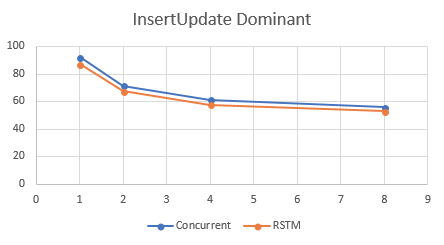
\includegraphics[scale=.6]{WriteDominatedConcurrent.png}
	\caption{(a) Write Dominant | Concurrent \& RTSM}
	\label{writeDom1}
\end{figure}

\begin{figure}[thpb]
	\centering
	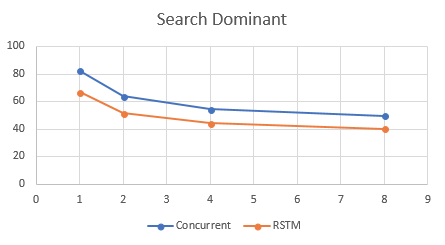
\includegraphics[scale=.6]{SearchDominatedConcurrent.png}
	\caption{(b) Search Dominant | Concurrent \& RTSM}
	\label{searchDom1}
\end{figure}

\begin{figure}[thpb]
	\centering
	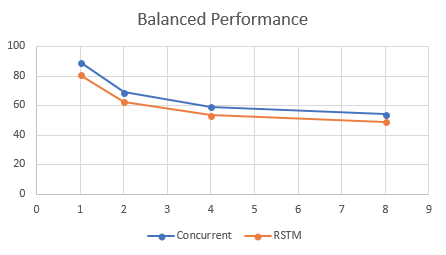
\includegraphics[scale=.6]{mixedWorkloadConcurrent.png}
	
	\caption{(c) Mixed Workload | Concurrent \& RTSM}
	\label{mixedWork1}
\end{figure}

\subsection{Experimental Results}
\textit{\textbf{Note:} These experimental results were aggregated from a previous iteration of our code. The code we have submitted is the progress that we have made since the experimentation to further our re-implementation of \cite{c1}'s proposed data structure.}

	\section{CONCLUSIONS}
	Our presentation of both the concurrent and transactional data structure implementations deriving from \cite{c1} demonstrates the linearizibility of the resulting C++ program. Searching in the Red-Black tree using these algorithms will be significantly less expensive due to the lack of helping. Modify operations that are performed in separate windows are able to execute concurrently without loss of correctness at any point because of the single word compare and swap instructions used when swapping out windows during a window transaction.

	\section*{APPENDIX}
	
	\begin{thebibliography}{99}
		
		\bibitem{c1} A. Natarajan, L. Savoie, \& N. Mittal 2013. 'Concurrent Wait-Free Red Black Trees'. The University of Texas at Dallas, Richardson, TX 75080, USA.
		\bibitem{c2} V. Kubushyn 2014. 'Concurrent Localized Wait-Free Operations on a Red Black Tree'. University of Nevada, Las Vegas.
		\bibitem{c3} J. H. Kim, H. Cameron, \& P. Graham 2006. 'Lock-Free Red-Black Trees Using CAS'. \textit{Concurrency and Computation: Practice and Experience}, 1-40.
		\bibitem{c4} J. Ma, 2003. 'Lock-Free Insertions on Red-Black Trees. MSc thesis. University of Manitoba.
		\bibitem{c5} J.J. Tsay \& H.C. Li 1994. 'Lock-Free Concurrent Tree Structures for Multiprocessor Systems'. \textit{Parallel and Distributed Systems, 1994}, 554-549. IEEE.
		\bibitem{c6} V.J. Marathe, M.F. Spear, C. Heriot, A. Acharya, D. Eisenstat, W.N. Scherer III \& M.L. Scott. 'Lowering the Overhead of Nonblocking Software Transactional Memory'. Computer Science Department, University of Rochester.
		\bibitem{c7} R.E. Tarjan 1985. 'Efficient Top-Down Updating of Red-Black Trees'. Computer Science Department, Princeton University, Princeton, NJ 08544. 
		\bibitem{c8} P. Chuong, F. Ellen, \& V. Ramachandran 2010. 'A Universal Construction for Wait-Free Transaction Friendly Data Structures'. In: \textit{Proceedings of the 22nd ACM Symposium on Parallelism in Algorithms and Architectures (SPAA)}. Thira, Santorini, Greece, pp. 335-344.
				
	\end{thebibliography}
	
	
	
	
\end{document}
